\chapter{Background}
\label{chap:backgnd}
\begin{abstractchap}
This chapter goes into detail about theoretical axes of this dissertation. First, we present language representations and specifically the three different types that interest us: lexical, syntactic and semantic. Secondly, we cover how we can infer relatedness among words based on the neighbors of each word. This intuition is expressed by the distributional hypothesis. Thirdly, we explain how  we can join words together through their common features by means of a graph-like structure. This structure is known as a language network. Fourth, we detail the techniques used in the multimedia literature to combine (or fuse) features coming from different sources and improve the performance of a knowledge-discovering system. In our work, instead of combining different multimedia sources, we combine diverse textual representations. Finally, we explain the (supervised and unsupervised) methods we employ to solve the NLP tasks at hand.
\end{abstractchap}
\minitoc

\section{Distributional Hypothesis}
The work we present in this thesis is prominently based on the distributional hypothesis (DH). This is also the case for the large majority of semantic approaches in NLP today. This context-analysis insight is usually credited primarily to \cite{harris1954}. The hypothesis is simple yet powerful: it can be formulated as "You shall know a word by the company it keeps." \cite{firth57synopsis}. More formally, it states that the similarity of meaning correlates with the similarity of the word's context distribution. It follows that the meaning of a word can be determined by the set of contexts in which it occurs in a corpus. Consequently, for two target words, the larger the number of shared contexts, the semantically closer these words are. 

\begin{figure}
\centering
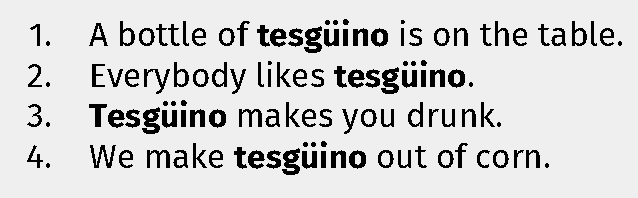
\includegraphics[width=.6\linewidth]{images/Chapitre2/tejuino.pdf}
\caption{Even though \textit{tesg\"{u}ino} is a relatively obscure word, from its context we can understand its an alcoholic drink made from corn.}
\label{fig:tejuino}
\end{figure}


Taking the classic example by \cite{nida1979componential}, shown in the four lines  in Figure \ref{fig:tejuino}, even if we do not know that the word tesg\"{u}ino (or tejuino) refers to a ceremonial corn beer consumed by the native people of the north of Mexico, we can infer, by looking at its context, that we are indeed referring to some sort of corn alcoholic beverage. We can then easily infer that tesg\"{u}ino is similar to other drinks such as tequila or mezcal.



Although we usually find in the literature that the work of Harris is the most important concerning the DH, we should note that the hypothesis rests on two theories  \cite{sahlgren2008distributional,turney2010}: the statistical semantics hypothesis \cite{booth1955machine}, and the  structuralism theory, as described by \cite{de1916course}. The former is important as it place the DH in a within a larger context. Broadly, it affirms that statistical patterns of human word usage can be employed to understand what people mean. The latter,  gives the DH a more robust approach towards the definition of what kind of distributional context should we use to determine similarities, as well as what does it the meaning of the contextual relations between words. In plain words Saussure's version of the structuralist theory indicates that the differences in the contexts of a word determine its role within a language system. 

To this end, Saussure proposed two kinds of context relations: syntagmatic and paradigmatic. Syntagmatic relations concern the context defined by words that co-occur in the text, such as collocations (multi-word expressions that occur frequently in a corpus) and colligations (relations between a lexical item and a grammatical category) \cite{verschueren2015handbook}. On the other hand, paradigmatic relations associate words according to whether they appear or not in the same context. These contexts define classic semantic relations such as synonymy-antonymy or hypernymy-hiponymy. Coupling both the DH with structuralist theory gives birth to the more refined definition of the distributional hypothesis, introduced by \cite{sahlgren2008distributional}: the refined distributional hypothesis. We note that this distinction, syntagmatic versus paradigmatic relations, is also more recently defined in \cite{schutze1993vector}. In their work, syntagmatic relations are called first-order co-occurrences, while paradigmatic relations  are referred to as secord-order co-occurrences.

\begin{figure}
\centering
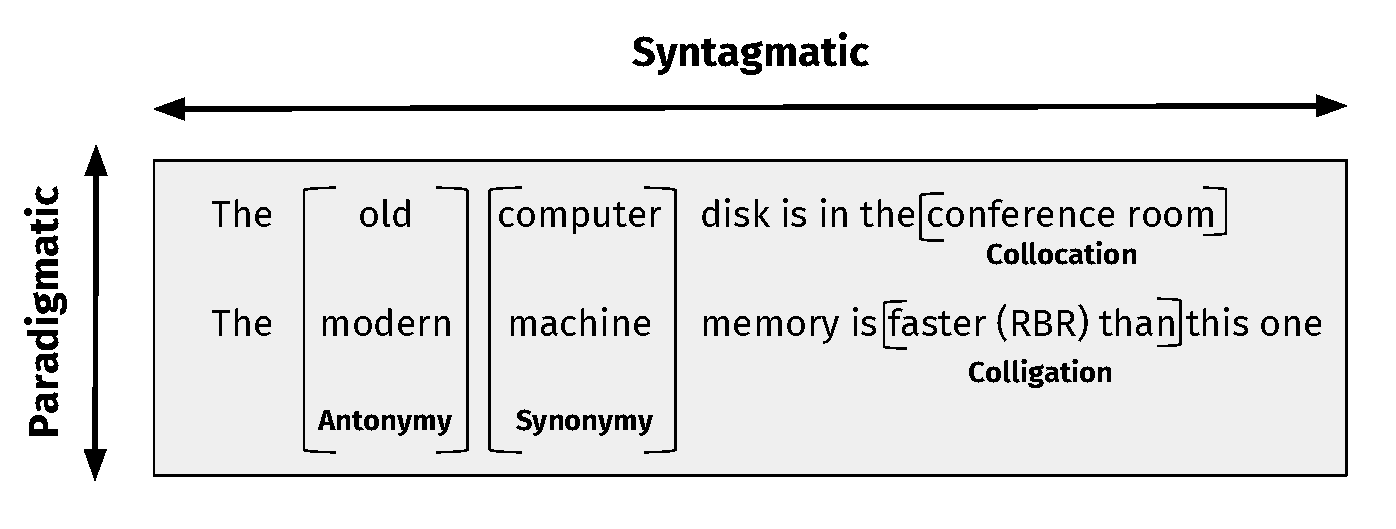
\includegraphics[width=\linewidth]{images/Chapitre2/sintagmatic_paradigmatic.pdf}
\caption{Examples of syntagmatic and paradigmatic contexts and their corresponding semantic relationships. Based on the examples by \cite{sahlgren2008distributional,piero2017}.}
\label{fig:sintagmatic_paradigmatic}
\end{figure}


An example of syntagmatic and paradigmatic relationships can be seen in Figure \ref{fig:sintagmatic_paradigmatic}. Vertically looking at the words,  \textit{old} and \textit{modern}, in the first and second phrase respectively,  share a paradigmatic context which leads to an antonym semantic relation. Something similar happens with words \textit{computer} and \textit{machine}, this time sharing a synonym relation. With respect to the syntagmatic relationships, horizontally looking at the words, we find the collocation \textit{conference room} in the first phrase, as well as the colligation in the second expression between the word \textit{than} usually preceded by a  comparative adverb (RBR), \textit{faster} in this case. 

In spite of Sahlgren's  distributional hypothesis definition, determining the types and meaning of semantic relations, obtained with distributional methods, is still an open challenge on distributional models and methods. Determining the specific type of semantic relation (e.g., synonymy, hyponymy, meronymy) is still an open issue in the community \cite{turney2010,fabre2015,perinet2015}. While distributional models can give us fast access  to semantic relations between words within a corpus, they are most of the times ambiguous relations. It is still our task, as users, to determine the type of semantic relations found, in the case these distinctions are needed by the NLP system  at hand.
% We note that our work does not delves into the study of the semantic relations but we use them to relate 

Distributional methods, based on the DH, have been used for a long time now \cite{JurafskyM09}, although computationally automatized since the 1990s \cite{perinet2015}. Being a mature research field, systems based on these distributional models are varied and cover a large range of NLP tasks being obviously most popular on semantic tasks \cite{bruni2014multimodal}. We do note that nowadays, they have somewhat resurfaced (although they really never went away) thanks to the recent re-introduction of word embeddings, or simply word distributional representations. In short, a word embedding, in the context of newer developments, is a vectorial representation  that "embeds" words into a low-dimensional space, usually generated either by means of some sort of matrix reduction \cite{lebret2013deep,levy2014neural} or by using neural networks \cite{Collobert2011,mikolov2013distributed}. These representations are usually obtained from very large bodies of text and they have shown to be quite effective for solving NLP tasks.

The actual implementation of a distributional model consists in three steps: (1) determine what type of context is going to be used, (2) chose a computable context representation, and (3) determine a weighting scheme  and a  relatedness measure.

\subsection{Types of Contexts}
We move now onto the description of what are the types of contexts commonly used while implementing a distributional model to represent words.  We cover two types: lexical co-occurrence and syntactical co-occurrence. In this work we will exclusively focus on on those two contexts. The first one describes a word's context based on its nearby words.  The second defines a word's context according to the syntactic relations between the word and its neighbors. We will use the example phrases in Figure \ref{fig:example_phrases} to illustrate the kind of contexts we will describe below. 
\begin{figure}
\centering
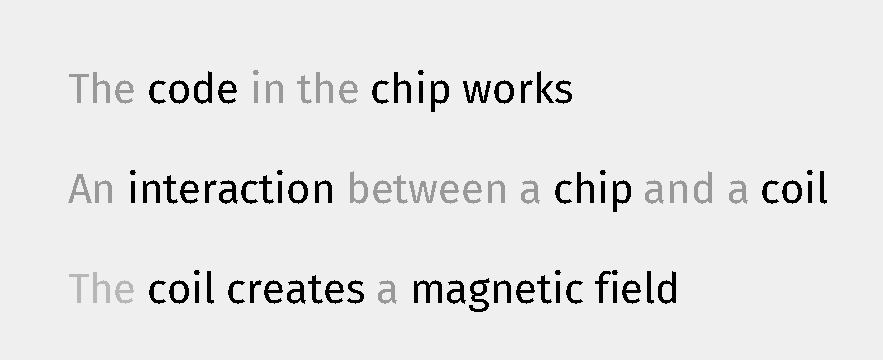
\includegraphics[width=0.7\linewidth]{images/Chapitre2/example_phrases.pdf}
\caption{Example text. Functional words are grayed-out. }
\label{fig:example_phrases}
\end{figure}

%todo Add as footnote the distinction between similarity and relatedness in Turney, Jurafsky, et al
%todo Define what is a target word (first time i talk about target word??)
%todo Add that a "Topical semantic relatedness" is obtained when context window is larger


\paragraph{Lexical Contexts}
Also called linear contexts, lexical contexts consist on those  words that co-occur with a given word in a predetermined neighborhood: either in a sentence, a paragraph or larger units of text such as full documents \cite{LevyG14,sahlgren2008distributional}. Nowadays, the lexical context is usually determined by a window of $n$ tokens to each side of the target word. As an example is shown in Table \ref{tab:exo_lexical_contxt}, where the context -2+2 of the words \textit{code}, \textit{chip}, and \textit{coil} is shown. The size of the context depends of course of the application of the system. Indeed, determining the size  is actually a quite empirical decision. Nonetheless, it seems that today the literature \cite{Daume2006,mikolov2013distributed,LevyG14,levy2014neural}  has settled for a two-words to the left and two-words to the right context window (plus the target word), otherwise represented as -2+2. \cite{sahlgren2006word} discusses  the motivations of selecting a window of a particular size. He notes that given the literature evidence,  a shorter context window (specifically a -2+2 window) is preferable for acquiring semantic information. In this sense, \cite{JurafskyM09} determines that generally the context size used lies between 1 and 8 words on each side, or 3 and 17 in total. In practical terms, the choice of the size  affects the scope of the semantic relatedness: the shorter the context, the more specific is the information about a target word, approaching syntactic relations. Furthermore, these relations are "stronger" in the sense of being semantically similar, we could in theory substitute one word for another as the shared relations are antony. On the contrary, the larger the window, the broader the information conferred by the context words. 



% Please add the following required packages to your document preamble:
% \usepackage{booktabs}
\begin{table}[]
\centering
\caption{Lexical contexts of the words \textit{code}, \textit{chip}, and \textit{coil} appearing in each one of the phrases on Figure \ref{fig:example_phrases}. The context is paradigmatic, the window being the word and 2 words to the left and right.}
\label{tab:exo_lexical_contxt}
\begin{tabular}{@{}ll@{}}
\toprule
Words & Lexical Context                        \\ \midrule
code  & code;\textbf{w+1}:chip; \textbf{w+2}:works                    \\
chip  & \textbf{w-2}:interaction; chip; \textbf{w+1}:coil \\
coil  & coil;\textbf{w+1}:creates; \textbf{w+2}:magnetic              \\ \bottomrule
\end{tabular}
\end{table}

Lexical co-occurrences are the most popular way to represent distributional contexts. They are easy to obtain as there is no need for external information except the input corpus itself. 
 




%\subsection{Lexical Representations}
%\subsection{Syntactic Representations}
%
\paragraph{Syntactic Contexts}

The second type of context depends on a more profound analysis of text. As its name implies, sytanctic contexts are based on the analysis (or parsing) of text in order to obtain sense from them. Lexical contexts are able to somehow take into account the order of appearance of words in a phrase. Still, words in a sentence are not related among them like a list: semantic information is indeed extracted from words themselves, however syntax highly affects the way information is combined into semantic structures. Words tend to form groups between themselves, called constituents or chunks, which relate to other constituents to form a single phrase unit \cite{bender2013linguistic}.

\subparagraph{Constituent Tree}
Indeed, constituents are  represented with tree structures aptly named  constituents parse tree, or simply parse tree (see Figure \ref{fig:exo1_constits}) \cite{JurafskyM09}. These trees actually represent the context-free grammars models that we use to describe the chunk structure. As such, the parse tree differentiates between terminal, pre-terminals and non-terminal nodes. Non-terminal nodes refer to chunk labels (e.g., noun phrases\footnote{This nomenclature is the most prevalent: the Penn Tree Bank annotation.}: \textit{NP}, verbal phrases: \textit{VP}, prepositional phrases: \textit{PRP}), pre-terminal nodes pertain to part of speech categories (e.g., determinants: \textit{DT}; adjectives: \textit{JJ}; nouns: \textit{NN}). Finally, terminal nodes indicate the word itself. 

%todo References, who is using constituents trees??
A constituents tree is illustrated in Figure \ref{fig:exo1_constits}. The image corresponds to the parse tree of the first phrase of the example in \ref{fig:example_phrases}: \textit{An interaction between a chip and a coil}. From the bottom-up,  looking at the node labeled \textit{chip}, we see it is a token of type noun (pre-terminal labeled \textit{NN}) and it belongs to a noun phrase (non-terminal \textit{NP}) which in turn belongs to a prepositional phrase (\textit{PP}) which finally is part of the main noun phrase of the sentence \textit{S}. Constituents usually include a word with a prominent role: the \textbf{head} of the constituent. In practical terms, the head (or governor) is the most important word in the chunk because it determines what kind of words (either a verb, an adjective, a noun, etc.) will be joining it within the constituent. 

The context that can be extracted from a constituency parse is similar to that of the lexical contexts, in that words themselves are part of the co-occurrent neighborhood. Yet, with the information from the parse tree, we can restrict the window to a chunk and heal consider only certain structural units. The context of \textit{code} and \textit{chip} of the parse  in Figure \ref{fig:exo1_constits} are shown in Table \ref{tab:exo_constits_contxt}. They consist simply in th non-functional words that co-occur with each word in a given constituent, in this case a noun phrase (NP).

\begin{figure}[t!]
	\begin{minipage}{\textwidth}
		\begin{minipage}{.9\textwidth}
			\centering
			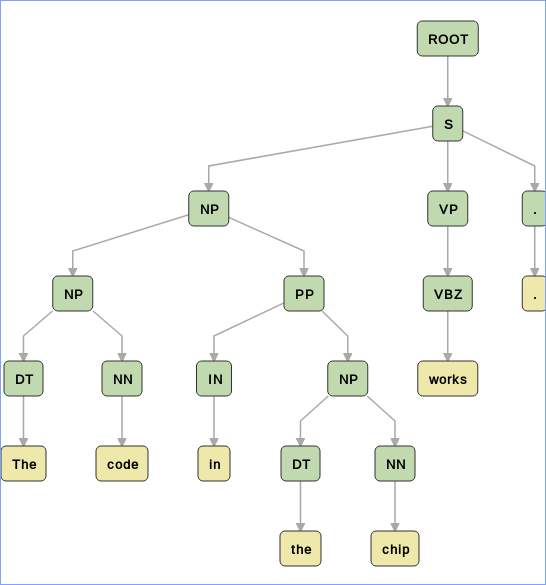
\includegraphics[width=0.7\linewidth]{images/Chapitre2/exo1_constits.png}
			\captionof{figure}{Constituents tree parse of the phrase \textit{The code in the chip works.}}
			\label{fig:exo1_constits}
		\end{minipage}
		\\
		\\
		\begin{minipage}{.9\textwidth}
			\centering
			\begin{tabular}{@{}ll@{}}
			\toprule
			Words & Lexical Context                        \\ \midrule
			code  & \textbf{NP}:chip                    \\
			chip  & \textbf{NP}:code \\
			\end{tabular}
			\captionof{table}{Syntactic contexts, based on the constituents tree in Figure \ref{fig:exo1_constits}, corresponding to the words \textit{code} and \textit{chip}, from the first phrase on Figure \ref{fig:example_phrases}.} 
			\label{tab:exo_constits_contxt}
		\end{minipage}
	\end{minipage}
\end{figure}

%TODO What is a grammar?
\subparagraph{Dependency Tree}
While  a parse tree represent the units existing within a sentence. As a complementary approach we can also formalize syntactic information with dependency trees. This time, the syntactic structure of a sentence is described in terms of words and asymmetric binary grammatical functions between these words   \cite{ClarkBook2010}. The trees are directed, all nodes are terminal and they represent words and they are linked following a direction from the head to its \textbf{modifier} (or dependent). An edge thus represent one of these dependency functions which are labeled  with tags that, just as PoS tags and chunk tags, describe what kind of relation exists between two words \cite{bird2006nltk}. For example, the Universal Dependencies\footnote{This set of tags share a large quantity of labels with the more classic Stanford Dependencies \cite{de2006generating,de2008stanford} tagset. Briefly, universal dependencies aim to develop cross-linguistically and cross-language consistent annotations  \cite{nivre2016universal}.} tagset \cite{nivre2016universal,schuster2016enhanced}, which we use in this work, includes tags such as  \textit{det}: determiner, the relation between a noun head (governor) and its determiner, \textit{nmod}: nominal modifier, the same but with a modifier, or \textit{conj}: conjunction, two elements connected by a conjunction.

To illustrate dependency trees, we can observe in Figure \ref{fig:exo1_dependences} the dependency parse of the same first used in the previous examples. In this particular case, the relation tags used are the "enhanced" universal dependencies by \cite{schuster2016enhanced}. The difference is that relations are made more explicit by collapsing them (reducing two relation edges into a single one)  and including the modifier  (or adjunct) directly into the label. Consequently, they can be more useful to determine the relatedness between words.

The context that can be extracted from dependency relations varies. Still, the usual consensus is to treat the relation as the triple it is: $(head, relation, dependent)$ and based on that extract a certain type of context. In the example of Figure \ref{fig:exo1_dependences}, a context of the word  \textit{chip}, according to \cite{Lin1997} would be: $(conj:and,coil,head)$. This indicates that \textit{chip} is connected to \textit{coil} by the conjunction \textit{and}. More recent context definitions, such as those of \cite{baroni2010distributional,LevyG14,Panchenko2017} also include the inverse relation a word participates in, i.e., if the target word is a dependent, its dependency relation is also included but indicated as "inverse".  Again, using the previous example with the  word \textit{chip}, the  contexts now would then be: interaction/nmod:between$^{-1}$;coil/conj:and . These contexts and other example can be seen in Table \ref{tab:exo_deps_contxt}.

\begin{figure}[!t]
 \begin{minipage}{\textwidth}
  \begin{minipage}{.9\textwidth}
    \centering
	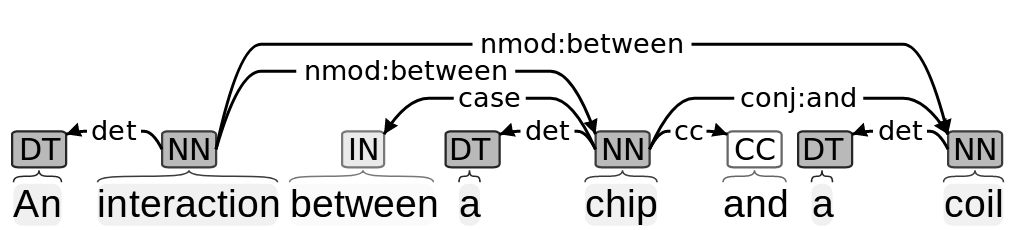
\includegraphics[width=0.9\linewidth]{images/Chapitre2/exo1_dependences.png}
    \captionof{figure}{Dependency tree parse of the phrase \textit{An interaction between a chip and a coil.}}
    \label{fig:exo1_dependences}
  \end{minipage}
  \\ 
  \\
  \begin{minipage}{.9\textwidth}
    \centering
		\begin{tabular}{@{}ll@{}}
		\toprule
		Words & Syntactic Context                        \\ \midrule
		interaction  &   coil/nmod:between; chip/nmod:between                   \\
		chip  & interaction/nmod:between$^{-1}$; coil/conj:and \\
		coil  & interaction/nmod:between$^{-1}$; chip/conj:and$^{-1}$      \\ \bottomrule
		\end{tabular}
		\captionof{table}{Syntactic contexts, based on the dependencies tree in Figure \ref{fig:exo1_dependences}, corresponding to the words \textit{interaction}, \textit{code}, and \textit{chip}, from the second phrase on Figure \ref{fig:example_phrases}} 
		\label{tab:exo_deps_contxt}
    \end{minipage}
  \end{minipage}
\end{figure}

Syntactic contexts are less used than their lexical counterpart in large part due to the process of obtaining the trees discussed before. While nowadays there are several software solutions able to extract this kind of information, the process is decidedly more complex than counting words in a lexical context setting. Furthermore, the information is not 100 \% accurate, as the systems are trained using human annotated banks of trees (called treebanks) which is in itself an ambiguous and hard process \cite{JurafskyM09,perinet2015}.  This difficulty stems yet another problem with syntactic information: syntactic parsers are not easily available for languages other than English and the rest of those in  the indo-european family. As a last downside, these contexts are known to generate sparse computational representations \cite{sahlgren2006word}. Still, syntactic contexts are shown to be able to contribute more information about word's relations than simple lexical contexts \cite{Lin1997,pado2003constructing,turney2010,baroni2010distributional,LevyG14,Panchenko2017}.

We have presented the two  main types of co-occurrence contexts that can represent a word in a corpus. In the next section we present the structures that allow mathematical and computational manipulation of the information provided by these contexts.







%\blindtext %1 %7 lineas x 8.3 =~ 60 lineas


\subsection{Vector Space Model}
%\paragraph{Vector Space Model}

The whole point of determining contexts, either lexical or syntactical, for a set of words in a corpus is to be able to assess how similar their meaning is among them. This assessment of relatedness thus need to be measured by a metric in order to determine its level. The way we measure the relatedness between words relies on well-known algebraic operations, such as the dot  product. In order to calculate a dot product we need vectors. It follows that to calculate relatedness among words we need to represent words by means of vectors, where each vector describe a word and each dimension a context of it. 

The Vector Space Model (VSM) consists in representing textual units in a multi-dimensional space. The textual units represented are not constrained to words themselves. We may describe co-occurrent features for documents, phrases, paragraphs, or other types \cite{manning1999foundations}. A matrix is used as the structure that holds each object and its context features. Indeed, in practical terms, a VSM is then an array of real-number vectors, where each one represent a text unit and the columns describes the co-occurrent contexts the word participates in. To illustrate  this, in Table \ref{tab:lexical_matrix} we represent words of the previous examples in a \textit{word space}. Each entry of this matrix (called a co-occurrence matrix) represent a weight that infers the importance of the row word (or target word) with respect to the column (context) co-occurrence in a given context, within an input corpus \cite{JurafskyM09}. That is, the word \textit{code}, co-occurs once with the context indicated by the second and third columns, which in turn correspond to the words \textit{chip} and \textit{works}.
%We note that some vector space models are not constrained to 2-dimensional matrices and leverage structures of larger dimensions \cite{baroni2010distributional}.

In the example, the weights consist merely in the frequency of co-occurrence of each word with each context. Indeed, there are still other two related parameters that affect the meaning extracted from a distributional model: the weight each cell in the matrix has, or how do each co-occurrence affect each word; and the similarity measure  between vectors we will use to determine the semantic relatedness among words. For a complete analysis on a wide range of parameters affecting vector space models, see \cite{baroni2010distributional,kiela2014systematic,levy2015improving}.



\begin{table}[]
\centering
\caption{Lexical contexts of the words appearing in the phrases of Figure \ref{fig:example_phrases}. The context is paradigmatic, the window being the complete phrase where the word occurs.}
\label{tab:lexical_matrix}
\begin{tabular}{@{}lrrrrrrrr@{}}
\toprule
       & $w_1$ & $w_2$ & $w_3$ & $w_4$ & $w_5$ & $w_6$ & $w_7$ & $w_8$ \\ \midrule
code$_{w_1}$        & 0    & 1    & 1     & 0           & 0    & 0       & 0        & 0     \\
chip$_{w_2}$        & 0    & 0    & 0     & 1           & 1    & 0       & 0        & 0     \\
works$_{w_3}$       & 1    & 1    & 0     & 0           & 0    & 0       & 0        & 0     \\
interaction$_{w_4}$ & 0    & 1    & 0     & 0           & 1    & 0       & 0        & 0     \\
coil$_{w_5}$        & 0    & 1    & 0     & 1           & 0    & 1       & 1        & 1     \\
creates$_{w_6}$     & 0    & 0    & 0     & 0           & 0    & 0       & 1        & 1     \\
magnetic$_{w_7}$    & 0    & 0    & 0     & 0           & 0    & 1       & 0        & 1     \\
field$_{w_8}$       & 0    & 0    & 0     & 0           & 1    & 1       & 1        & 0     \\ \bottomrule
\end{tabular}
\end{table}

%todo slides the word-embeddings.pdf page 34 would be cool to put in this chap
%1 weighting
\paragraph{Matrix Weights}

The weight is an important parameter in the creation of a VSM for a NLP application. Weights can be binary, simply  indicating presence or absence. They can count the number of co-occurrences of a word and the context, their absolute frequency. Weights may also be a type of discriminative measure that usually tries to give more importance to those contexts that co-occur more frequently with the target word while being less frequent  with the rest of the words in the text \cite{JurafskyM09,ClarkBook2010}.  

Point-wise Mutual Information (PMI) \cite{Church1990} and Positive Point-wise Mutual Information (PPMI) \cite{niwa1994co} are two popular choices to weight terms in a co-occurrence matrix \cite{turney2010,JurafskyM17}. We describe both of them below.

Given a co-occurrence matrix M, containing $W$ words (rows) and $C$ contexts (columns), where $f_{ij} \in \mathbb{R}^{W\times V}$ denotes the frequency of  target word $w_i$ frequency in the context $c_j$ , i.e., how many times they both co-occur. $N=\sum_{i=1}^W\sum_{j=1}^Cf_{ij}$ represents the sum of all the matrix cells. PMI is defined as:
\begin{equation} \label{eq:pmi}
PMI(w_i,c_j) = \log\dfrac{P(t_{ij}|c_j)}{P(t_{ij})P(c_j)}
\end{equation}
where  $P(t_{ij}|c_j)=\dfrac{f_{ij}}{N}$ tells us how many times the word and the context appeared together, normalized by the total context frequency. $P(t_{ij})= \dfrac{f_{ij}}{N}$, and $P(c_j)=\dfrac{f_j}{N}$. The ratio gives us an estimate of how much more the target and context co-occur than we expect by chance.

While PMI is often used as a weighting choice, it has three main downsides \cite{JurafskyM17,levy2015improving}: (1) PMI is biased towards co-occurrences of rare events: a low-frequency context $c$ co-occurring with any word $w$ will yield a large PMI. Also (2), PMI may yield negative values, which would indicate a certain level of semantic "unrelatedness", which is not a  very intuitive concept. And (3),  if a context and a target word are not observed together (something that is very possible to happen because the co-occurrence matrix is sparse, we will look into that in the following paragraphs), the denominator of \ref{eq:pmi} is zero and thus $PMI_{ij}$ becomes undefined. 

To solve the first issue, \cite{levy2015improving} proposes a smoothed version of PMI, defined as:
\begin{equation} \label{eq:pmi_levy}
PMI_\alpha(w_i,c_j) = \log\dfrac{P(t_{ij}|c_j)}{P(t_{ij})P_\alpha(c_j)}
\end{equation}

with $P_\alpha(c_j) = \dfrac{f_j^\alpha}{N^\alpha}$, where $\alpha$ is a smoothing parameter that affects the contexts counts in order to alleviate the bias of PMI towards rare contexts co-occurrences : the probability of a low-frequency context $c_j$ will be larger thanks to $\alpha$, which makes the denominator of \ref{eq:pmi_levy} larger, which in turns make PMI$_\alpha$ smaller. Thus, addressing the bias for all words when co-occurring with a low-frequency context.


The second and third inconvenient are resolved by using Positive Point-wise Mutual Information (PPMI). PPMI simply replaces all values lower than zero (including $-\infty$) by a zero:
\begin{equation} \label{eq:ppmi}
PMI(w_i,c_j) = \max(PMI(w_i,c_j), 0)
\end{equation}
%2 similarity
\paragraph{Defining Vector Similarity}
%3 sparsity (long, important paragraph)
The second parameter to consider after weighting the co-occurrence matrix is how to actually determine the similarity between two word vectors.

As with weighting schemes, there are multiple metrics \cite{ClarkBook2010,kiela2014systematic,clark2015vector} used in the literature to determine the similarity between two vectors. We will focus on two that are of interest to this thesis: cosine and Jaccard similarity. More types of metrics and their comparison can be found in the previously cited literature. While there does not seem to be a single best measure of similarity, we usually use the cosine similarity, as it naturally can deal with real-valued vectors. On the other hand, when dealing with binary presence-absence vectors, it is more common to use Jaccard. 

\subparagraph{Cosine Similarity}
The cosine similarity determines the angle between two multidimensional vectors. It is simply defined as the dot product between two vectors, normalized by the multiplication of their Euclidean length \cite{Manning2008}. The cosine similarity is bounded between $[0,1]$, yet we usually interpret the result in the positive space, where 0 means there is an angle of $90^\circ$ between the two word vectors, thus  no similarity at all; and 1 means there is no angle between them, so they are completely similar. Furthermore, if the weights of the matrix are non-negative values, the cosine similarity is bounded to the range $[0,1]$, The cosine similarity is defined as:
\begin{equation}
sim_{cosine}(\overrightarrow{w_1},\overrightarrow{w_2})  =  \dfrac{\overrightarrow{w_1}  \cdot \overrightarrow{w_2}}{||\overrightarrow{w_1}||\,||\overrightarrow{w_2}||} = \dfrac{\sum_{i=1}^Cw_{1_i}\times w_{2_i} }{\sqrt{\sum^C_{i=1}w_{1_i}^2}\sqrt{\sum^C_{i=1}w_{2_i}^2}}
\end{equation}

\subparagraph{Jaccard Index}
Also named the Tanimoto index, the Jaccard index \cite{jaccard1908nouvelles} determines the similarity between binary vectors, it is defined, in terms of dot products:

\begin{equation}
sim_{Jaccard}(\overrightarrow{w_1},\overrightarrow{w_2}) = \dfrac{\overrightarrow{w_1} \cdot \overrightarrow{w_2}}{||\overrightarrow{w_1}||^2+||\overrightarrow{w_2}||^2 - \overrightarrow{w_1}\cdot\overrightarrow{w_2}}
\end{equation}
In terms of sets, the Jaccard index simply calculates the ratio between the intersection of two word vectors divided by their union. We present the dot product version because it is easier to implement computationally with that formulation.


\paragraph{Data Sparsity on VSM}

Representing word's contexts as multidimensional  vectors is indeed a straight-forward, simple and  yet powerful method to transform textual data into actionable structures. The model links  textual information, in te form of words and contexts, with the methods used in machine learning.

Nonetheless, there is an important issue that needs to be considered when dealing with vector space models. Indeed data sparsity 



%
%
%
%
%
%\section{Vector Space Model and Graph-based representations}
%\subsection{Vector Space Model}
%\subsection{Graph-based Models}
%
%
%
%\section{Supervised and Unsupervised Methods}
%\subsection{Supervised Methods}
%\subsubsection{Logistic Regression}
%\subsubsection{Structured Perceptron}
%\subsection{Unsupervised Methods}
%\subsubsection{Spectral Clustering}
%
%\section{Word Sense Induction and Disambiguation}
%\section{Named Entity Recognition}

%++++++++++++++++++++++++++++++++++++++++++++++++++++++++++++++++++++++++++++++++++++++++++++++++++



